\chapterWithSubtitle{Reductions}{April 15, 2021}

\section{Intractability and Lower Bounds}

\subsection{Turing Machines and Church-Turing Thesis}
\begin{itemize}
    \item Turing defined TMs as a machine model of computation.
    \item \textbf{Church-Turing Thesis}: any function that is computable can be computed by TMs.
    \item \textbf{Efficient Church-Turing Thesis}: any function that is computable can be computed by TMs with only a polynomial slow-down.
\end{itemize}

\subsection{Computability and Complexity Theory}
\begin{itemize}
    \item What function can and cannot be computed by TMs?
    \item What functions/problems can and cannot be solved efficiently?
    \item There are foundational questions about computation.
    \item Are we not able to figure out a solution or does a solution not exist?
\end{itemize}

\subsection{Lower Bounds and Impossibility Results}
\begin{itemize}
    \item Proving that a given problem cannot be solved (efficiently) on a TM, is difficult. 
    \item It is difficult to calculate a lower bound on a problem and algorithms can be very non-trivial.
\end{itemize}

\subsection{Reductions to Prove Intractability}
\begin{itemize}
    \item There is a general methodology to prove impossibility results:
    \begin{itemize}
        \item Start with some known hard problem $X$.
        \item Reduce $X$ to some problem $Y$.
    \end{itemize}
    \item If $Y$ can be solved, then so can $X$. Thus $Y$ is also hard.
    \item We can hard problems given by some clever person (Cantor/Gödel/Turing/Cook/Levin...) who estabilshed the hardness of a fundamental problem.
    \item We assume that some core problem is hard because we have not been able to solve it for a long time. This leads to conditional results.
\end{itemize}

\subsection{Decision Problems, Languages, Terminology}
\begin{itemize}
    \item When proving hardness, we limit attention to decision problems.
    \begin{itemize}
        \item A decision problem $\Pi$ is a collection of instances (strings).
        \item For each instance $I$ of $\Pi$, the answer is either YES or NO.
        \item Equivalently, a boolean function $f_\Pi: \sum^\ast \rightarrow \{ 0, 1 \}$ where $f(I) = 1$ if $I$ is a YES instance, and $f(I)) = 0$ if $I$ is a NO instance.
        \item Equivalently, a language $L_\Pi = \{ I \mid \text{$I$ is a YES instance} \}$.
    \end{itemize}
    \item We distinguish $I$ from the encoding $\langle I \rangle$.
    \begin{itemize}
        \item $n$ is an integer. $\langle n \rangle$ is the encoding of $n$ in some format (could be unary, binary, decimal, etc.).
        \item $G$ is a graph. $\langle G \rangle$ is the encoding of $G$ is some format.
        \item $M$ is a TM. $\langle M \rangle$ is the encoding of TM as a string according to some fixed convention.
    \end{itemize}
\end{itemize}

\section{Reductions}

\subsection{Reductions for Decision Problems and Languages}
\begin{itemize}
    \item For languages $L_x, L_y$, a reduction from $L_x$ to $L_y$ is an algorithm with input $w \in \sum^\ast$ and output $w' \in \sum^\ast$ such that $w \in L_x \iff w' \in L_y$.
    \item For decision problems $X, Y$, a reduction from $X$ to $Y$ is an algorithm with input $I_X$, an instance of $X$, and an output $I_Y$, and instance of $Y$, such that $I_X \text{ is a YES instance of } X \iff I_Y \text{ is a YES instance of } Y$
    \begin{itemize}
        \item $\mathcal{R}$: Reduction $X \rightarrow Y$
        \item $\mathcal{A}_Y$: algorithm for $Y$:
        \item The new algorithm $\mathcal{A}_X$ for $X$:
        \item[] \lstinputlisting{lecture21/code/reduction.sudo}
    \end{itemize}
    \item[] \begin{center}
        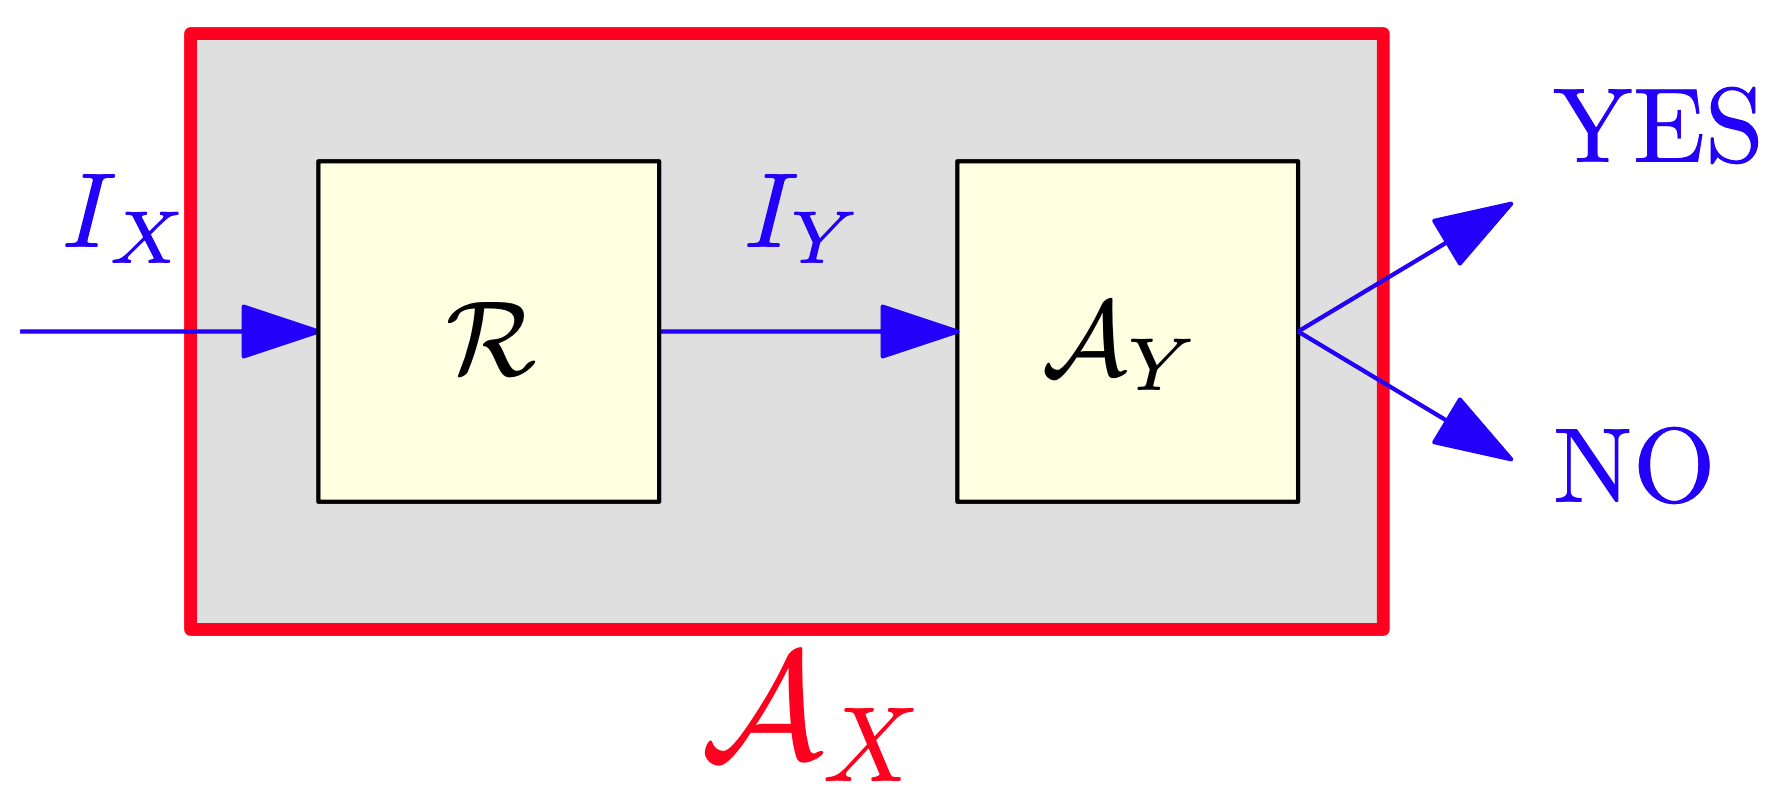
\includegraphics[width=0.5\textwidth]{lecture21/images/reduction.jpg}
    \end{center}
    \item If $\mathcal{R}$ and $\mathcal{A}_Y$ are polynomial time algorithms, then $\mathcal{A}_X$ is also polynomial time.
    \item The running time of $\mathcal{A}_X$ is $O(R(n) + Q(R(n)))$.
    \begin{itemize}
        \item $R(n)$: running time of $\mathcal{R}$.
        \item $Q(n)$: running time of $\mathcal{A}_Y$.
        \item If $I_X$ has size $n$, $\mathcal{R}$ creates an instance $I_Y$ of size at most $R(n)$.
        \item $\mathcal{A}_Y$'s time on $I_Y$ is by definition at most $Q(\left|I_Y\right|) \leq Q(R(n))$.
    \end{itemize}
\end{itemize}

\subsection{Notation and Implication of Reductions}
\begin{itemize}
    \item If Problem $X$ reduces to Problem $Y$, we write $X \leq Y$.
    \item If Problem $X$ reduces to Problem $Y$ where the reduction $\mathcal{R}$ is an efficient (polynomial-time algorithm), we write $X \leq_P Y$.
    \item Algorithmic Implications:
    \begin{itemize}
        \item If $X \leq Y$ and $Y$ has an algorithm, then $X$ has an algorithm.
        \item If $X \leq_P Y$ and $Y$ has a polynomial-time algorithm, then $X$ has a polynomial-time algorithm.
    \end{itemize}
    \item Hardness Implications:
    \begin{itemize}
        \item If $X \leq Y$ and $X$ does not have an algorithm, then $Y$ does not have an algorithm.
        \item If $X \leq_P Y$ and $X$ does not have a polynomical-time algorithm, then $Y$ does not have a polynomical-time algorithm.
    \end{itemize}
    \item $X \leq Y$ and $Y \leq Z$ implies that $X \leq Z$. Similarly $X \leq_P Y$ and $Y \leq_P Z$ implies $X \leq_P Z$.
\end{itemize}

\section{Examples of Reduction}

\subsection{Independent Sets and Cliques}
\begin{itemize}
    \item Given a graph $G = (V, E)$, $V' \subseteq V$ is a
    \begin{itemize}
        \item \textbf{Independent Set}: no two vertices of $V'$ are connected by an edge of $G$.
        \item \textbf{Clique}: every pair of vertices in $V'$ is connected by an edge of $G$.
    \end{itemize}
    \item Independent Set Problem
    \begin{itemize}
        \item \textit{Instance}: A graph $G$ and an integer $k$
        \item \textit{Question}: Does $G$ have an independent set of size greater than $k$?
    \end{itemize}
    \item Clique Problem
    \begin{itemize}
        \item \textit{Instance}: A graph $G$ and an integer $k$
        \item \textit{Question}: Does $G$ have a clique of size greater than $k$?
    \end{itemize}
    \item Reduction given $\langle G, k \rangle$ outputs $\langle \overline{G}, k \rangle$ where $\overline{G}$ is the complement of $G$. $\overline{G}$ has an edge $uv \iff uv$ is not an edge of $G$.
    \item An independent set of size $k$ in $G$ $=$ A clique of size $k$ in $\overline{G}$.
    \item Independent Set $\leq_P$ Clique.
    \begin{itemize}
        \item If we have an algorithm for Clique, then we have an algorithm for Independent Set.
        \item The reduction is efficient. Hence, if we have a polynomial-time algorithm for Clique, then we also have a polynomial-time algorithm for Independent Set.
        \item Clique is at least as hard as Independent Set.
    \end{itemize}
    \item The Independent Set problem is at least as hard as the Clique Problem (Clique $\leq$ Independent Set).
    \begin{itemize}
        \item $I_X = \langle G \rangle$
        \item $A_X = \text{Clique}$
        \item $I_Y = \langle \overline{G} \rangle$
        \item $A_Y = \text{Independent Set}$
        \item $R: \overline{G} = \{ V, \overline{E} \}$
    \end{itemize}
    If we let the independent set problem be $\mathcal{A}_X$ and the clique problem be $\mathcal{A}_Y$, $\mathcal{A}_X$ can be reduced so $\mathcal{A}_Y$ so $X \leq Y$.
\end{itemize}

\subsection{Independent Set and Vertex Cover}
\begin{itemize}
    \item \textbf{Vertex Cover}: For graph $G = (V, E)$, $S \subseteq V$ is a vertex cover if for every $e \in E$, there is at least one endpoint in $S$.
    \item Vertex Cover Problem
    \begin{itemize}
        \item \textit{Input}: A graph $G$ and integer $k$
        \item \textit{Goal}: Is there a vertex cover of size $\leq k$ in $G$?
    \end{itemize}
    \item The complement of the vertex set must be an independent set. If two vertices from the complement of a vertex set had an edge between them, one of them would need to be in the vertex set, and that would be a contradiction.
    \item Independent Set $\leq_P$ Vertex Cover.
    \begin{itemize}
        \item Let $G$, a graph with $n$ vertices, and an integer $k$ be an instance of the Independent Set problem.
        \item Our reduction, given $\langle G, k \rangle$ as an instance of the Independent Set, returns $\langle G, n - k \rangle$ as an instace of Vertex Cover. 
        \item $G$ has an independet set of size $\geq k$ if and only if $G$ has a vertex cover of size $\leq n - k$ which proves correctness.
        \item The reduction is efficient.
        \item Therefore Independent Set $\leq_P$ Vertex Cover. Also Vertex Cover $\leq_P$ Independent Set.
    \end{itemize}
\end{itemize}

\section{Reasoning about Programs}

\subsection{DFA Accepting a String}
\begin{itemize}
    \item \textit{Problem}: Given DFA $M$ and a string $w \in \sum^\ast$, does $M$ accept $w$?
    \begin{itemize}
        \item Instance: $\langle M, w \rangle$.
        \item Algorithm: given $\langle M, w \rangle$, output YES if $M$ accepts $w$, or else output NO.
    \end{itemize}
    \item We can simulate $M$ on $w$ and output $YES$ if $M$ reaches a final state.
\end{itemize}

\subsection{NFA Accepting a String}
\begin{itemize}
    \item \textit{Problem}: Given NFA $N$ and a string $w \in \sum^\ast$, does $N$ accept $w$?
    \begin{itemize}
        \item Instance: $\langle N, w \rangle$.
        \item Algorithm: Given $\langle N, w \rangle$, output YES if $N$ accepts $w$, or else output NO.
    \end{itemize}
    \item We can convert $N$ to an equivalent DFA $M$ and use the previous algorithm.
    \item Hence, we use a reduction that takes $\langle N, w \rangle$ to $\langle M, w \rangle$.
    \item The reduction is not efficient as $\left| M \right|$ is exponential in $\left| N \right|$ in the worst case.
\end{itemize}

\subsection{Reasoning about TMs/Programs}
\begin{itemize}
    \item $\langle M \rangle$ is an encoding of a TM $M$. Equivalently, think of $\langle M \rangle$ as the code of a program in some high-level programming language.
    \item There are three related problems:
    \begin{itemize}
        \item Given $\langle M \rangle$, does $M$ halt on blank input? (Halting Problem)
        \item Given $\langle M, w \rangle$, does $M$ halt on input $w$?
        \item Given $\langle M, w \rangle$, does $M$ accept $w$? (Universal Language)
    \end{itemize}
    \item \textbf{Turing Theorem}: All the three problems are undecidable. There exists no such algorithm/program/TM.
\end{itemize}
